\documentclass[twoside,10pt]{article}
\usepackage{amsmath,amsfonts,amsthm,fullpage,amssymb}
%\usepackage{mymath}
\usepackage{algorithm,amsmath,amssymb}
\usepackage{algorithmic}
\usepackage{graphicx, color}
\usepackage{url}
\usepackage[most]{tcolorbox}


\begin{document}


\title{ISYE 6740 Homework 6\\ 
Fall 2020\\
\small Total 100 points.}
\date{}
\author{Shasha Liao}
\maketitle



%As usual, please submit a report with sufficient explanation of your answers to each the questions, together with your code, in a zip folder.

%----------------------------------------------------------------------------------



\begin{enumerate}


\item  {\bf AdaBoost.} (30 points)

Consider the following dataset, plotting in the following figure. The first two coordinates represent the value of two features, and the last coordinate is the binary label of the data.
\begin{equation*}
\begin{split}
&X_1 = (-1, 0, +1), X_2 = (-0.5, 0.5, +1), X_3 = (0, 1, -1), X_4 = (0.5, 1, -1), \\
&X_5 = (1, 0, +1), X_6 = (1, -1, +1), X_7 = (0, -1, -1), X_8 = (0, 0, -1).
\end{split}
\end{equation*}

In this problem, you will run through $T = 3$ iterations of AdaBoost with decision stumps (as explained in the lecture) as weak learners.

\begin{enumerate}
\item (15 points) For each iteration $t = 1, 2, 3$, compute $\epsilon_t$, $\alpha_t$, $Z_t$, $D_t$ by hand (i.e., show the calculation steps) and draw the decision stumps on the figure (you can draw this by hand). 
\begin{tcolorbox}[breakable,enhanced]
\textbf{Solution:}
m = 8
\begin{center}
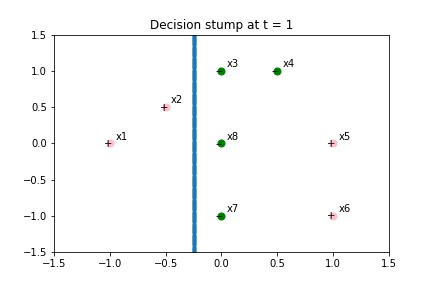
\includegraphics[width =0.5 \textwidth]{images/time1.jpg} 
\end{center}
\begin{itemize}


\item[t=1:] 
$D_1 = \frac 1 m = \frac 1 8 = 0.125 $ for all $i = 1, ..., 8.$ \\

$h_1(x; w_1, b_1) = sign(h_1(x; -1, -.25)) = sign(- x_1 - 0.25) $\\

$\epsilon_1 = \sum_{i=1}^m D_1(i) \mathbb{I}\{y^i \neq h_1(x^i)\} = \frac 1 8 * 2 = \frac 1 4 $\\

$\alpha_1 = \frac 1 2 \ln(\frac{1-\epsilon_1}{\epsilon_1}) = \frac 1 2 \ln(3)  \approx 0.549$

\begin{center}
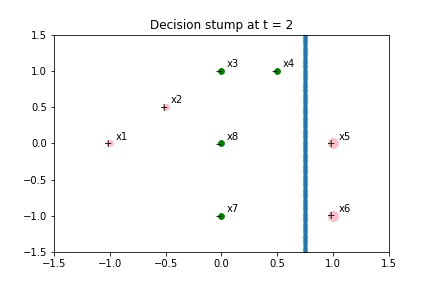
\includegraphics[width =0.5 \textwidth]{images/time2.jpg} 
\end{center}
\item[t=2:]
$Z_1 = \sum_{i=1}^m D_1(i)e^{-\alpha_1 y^i h_1(x^i)} = \frac{1}{8} e^{-\frac 1 2 \ln 3} * 6 + \frac{1}{8} e^{\frac 1 2 \ln 3} * 2 \approx 0.866 $ \\

$D_2(i) = \frac{D_1(i)}{Z_1}e^{-\alpha_1 y^i h_1(x^i)} \approx \left\{ \begin{array}{lcr} \frac 1 {8 * 0.866} e^{-\frac 1 2 \ln 3}  \approx 0.083 &\mbox{ if }&  i \neq 5,6  \\ \frac 1 {8 * 0.866} e^{\frac 1 2 \ln 3} \approx 0.250 &\mbox{ if }& i \in \{5,6\}\end{array}\right.$\\

We choose $h_2(x)$ to maximize $\sum_{i=1}^m D_2(i)y^i h_2(x^i)$: \\ 
$h_2(x; w_2, b_2) = sign(h_2(x; 1, -.75)) = sign( x_1 - 0.75) $\\

$\epsilon_2 = \sum_{i=1}^m D_2(i) \mathbb{I}\{y^i \neq h_2(x^i)\} \approx 0.083 * 2 \approx 0.167 $\\

$\alpha_2 = \frac 1 2 \ln(\frac{1-\epsilon_2}{\epsilon_2}) \approx 0.805$


\begin{center}
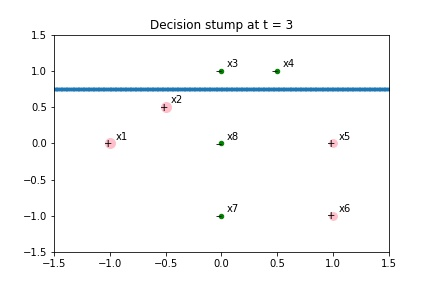
\includegraphics[width =0.5 \textwidth]{images/time3.jpg} 
\end{center}
\item[t=3:]
$Z_2 = \sum_{i=1}^m D_2(i)e^{-\alpha_2 y^i h_2(x^i)} = \sum_{i\in\{1,2\}} D_2(i)e^{\alpha_2} + \sum_{i\notin \{1,2\}} D_2(i)e^{-\alpha_2}  \approx 0.745 $ \\

$D_3(i) = \frac{D_2(i)}{Z_2}e^{-\alpha_2 y^i h_2(x^i)} \approx \left\{ \begin{array}{lcr} \frac {0.083} {0.745} e^{0.805}  \approx 0.250 &\mbox{ if }&  i \in \{1,2\}  \\ 

\frac {0.250} {0.745} e^{-0.805} \approx 0.150 &\mbox{ if }& i \in \{5,6\} \\

\frac {0.083} {0.745} e^{-0.805} \approx 0.050 &\mbox{ if }& i \in \{3,4,7,8\}  \end{array}\right.$\\

We choose $h_3(x)$ to maximize $\sum_{i=1}^m D_3(i)y^i h_3(x^i)$: \\ 
$h_3(x; w_3, b_3) = sign(h_3(x; -1, 0.75)) = sign( - x_2 + 0.75) $\\

$\epsilon_3 = \sum_{i=1}^m D_3(i) \mathbb{I}\{y^i \neq h_3 (x^i)\} \approx 0.050 * 2 =  0.100 $\\

$\alpha_3 = \frac 1 2 \ln(\frac{1-\epsilon_3}{\epsilon_3}) \approx 1.099$

$Z_3 = \sum_{i=1}^m D_3(i)e^{-\alpha_3 y^i h_3(x^i)} = \sum_{i\in\{3,4\}} D_3(i)e^{\alpha_3} + \sum_{i\notin \{3,4\}} D_3(i)e^{-\alpha_3}  \approx 0.6.$

\end{itemize}
\end{tcolorbox}
\newpage
\item (15 points) What is the training error of this AdaBoost? Give a short explanation for why AdaBoost outperforms a single decision stump.
%\vspace{-.2in}
%\begin{figure}[h!]
%\begin{center}
%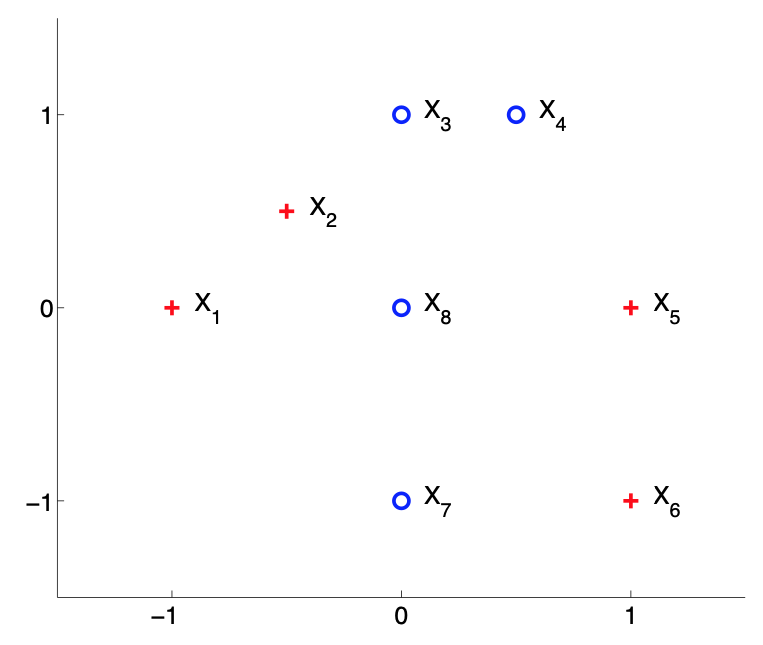
\includegraphics[width =.4 \textwidth]{hw}
%\end{center}
%\caption{ A small dataset, for binary classification with AdaBoost.}
%\end{figure}
%\vspace{-.3in}
%begin{tcolorbox}[breakable,enhanced]
\begin{tcolorbox}[breakable,enhanced]
\textbf{Solution:} The combined classifier is 
\begin{align*}
f_3(x) &= sign(\alpha_1 f_1(x) + \alpha_2 f_2(x) + \alpha_3 f_3(x)) \\
& = sign(0.549 * sign(-x_1 - 0.25) + 0.805 * sign(x_1 - 0.75) + 1.099 * sign(-x_2 + 0.75))
\end{align*}
where $x = (x_1, x_2)$. \\

After some calculation, we found the training error is $0$. The reason why AdaBoost outperforms a single decision stump is that AdaBoost combined a sequence of simple decision stumps to correct the mistakes the previous decision stumps made. The combined decision stumps can have complicated decision boundaries while simple stump can only have linear decision boundary.  

\end{tcolorbox}
\begin{table}
\begin{center}
\caption{Values of AdaBoost parameters at each timestep.}
\vspace{0.1in}
\begin{tabular}{|c|c|c|c|c|c|c|c|c|c|c|c|}\hline
t & $\epsilon_t$ & $\alpha_t$ & $Z_t$ & $D_t(1)$ & $D_t(2)$ & $D_t(3)$ & $D_t(4)$ & $D_t(5)$ & $D_t(6)$ & $D_t(7)$ & $D_t(8)$ \\\hline
1 & 0.250 & 0.549 & 0.866 &0.125 &0.125 &0.125 &0.125 & 0.125&0.125 &0.125 & 0.125\\
2 & 0.167 & 0.805 & 0.745 & 0.083 & 0.083 & 0.083 & 0.083 & 0.250 & 0.250 & 0.083 & 0.083 \\
3 & 0.100 & 1.099 & 0.600 & 0.250 & 0.250 & 0.050 & 0.050 & 0.150 & 0.150 & 0.050 & 0.050 \\\hline
\end{tabular}
\end{center}
\end{table}

\end{enumerate}
%\end{tcolorbox}
\clearpage 

\item{\bf Linear regression: bias-variance tradeoff, CV, and variable selection} (30 points)


Consider a dataset with $n$ data points $(x^i, y^i)$, $x^i \in \mathbb R^n$, following from the following linear model:
\[
y^i =  {\beta^*}^T x^i + \epsilon^i, \quad i = 1, \ldots, m,
\]
where $\epsilon^i$ are i.i.d. Gaussian noise with \textcolor{red}{zero mean and variance $\sigma^2$}, and $\beta^*$ is the true parameter. Consider the ridge regression as follows:
\begin{equation} \label{1}
\hat \beta(\lambda) 
= \arg\min_{\beta}
\left\{
\frac 1 m \sum_{i=1}^m (y^i - {\beta}^T x^i)^2 + \lambda \|\beta\|_2^2
\right\},
\end{equation}
where $\lambda \geq 0$ is the regularized parameter. 
\begin{enumerate}
\item (5 points) Find the closed form solution for $\hat \beta(\lambda)$ and its distribution conditioning on $\{x^i\}$ (i.e., treat them as fixed).
\begin{tcolorbox}[breakable,enhanced]
\textbf{Solution:} Denote $$L(\beta) := \frac 1 m \sum_{i=1}^m (y^i - {\beta}^T x^i)^2 + \lambda \|\beta\|_2^2.$$
Then 
\begin{align*}
\frac{\partial{L(\beta)}}{\partial \beta} & = \frac 2 m \sum_{i=1}^m (-x^i) (y^i - {\beta}^T x^i)+ 2\lambda \beta \\
& = - \frac 2 m \sum_{i=1}^m x^i y^i  +  \frac 2 m \sum_{i=1}^m x^i {\beta}^T x^i + 2\lambda \beta \\
& = - \frac 2 m \sum_{i=1}^m x^i y^i  +  \frac 2 m \sum_{i=1}^m x^i (x^i)^T {\beta}  + 2\lambda \beta \\
& =  -\frac 2 m Xy + \frac 2 m XX^T \beta + 2\lambda \beta. \\
\end{align*}
where $X = [x^1,x^2 ..., x^m] \in \mathbb{R}^{n\times m}$ and $y = (y^1, y^2, ..., y^m)^T \in \mathbb{R}^{m\times 1}$.\\

Setting $$\frac{\partial{L(\beta)}}{\partial \beta}=-\frac 2 m Xy + \frac 2 m XX^T \beta + 2\lambda \beta  = 0$$
gives us $$\hat{\beta}(\lambda) = \left( \frac 1 m XX^T + \lambda I \right)^{-1} \left(\frac 1 m Xy\right).$$

Since $$y^i =  {\beta^*}^T x^i + \epsilon^i, \quad i = 1, \ldots, m,$$
we know $$y = X^T \beta^* + \epsilon$$
where $\epsilon = (\epsilon^1, \epsilon^2, ..., \epsilon^m)^T.$

Therefore, 
\begin{align*}
\hat{\beta}(\lambda) &=  \left( \frac 1 m XX^T + \lambda I \right)^{-1} \left(\frac 1 m X(X^T \beta^* + \epsilon) \right) \\
& =  \left( \frac 1 m XX^T + \lambda I \right)^{-1} \left(\frac 1 m XX^T \beta^* + \frac 1 m X\epsilon \right) \\
& =  \frac 1 m \left( \frac 1 m XX^T + \lambda I \right)^{-1}  XX^T \beta^* + \frac 1 m \left( \frac 1 m XX^T + \lambda I \right)^{-1}  X\epsilon  \\
\end{align*}
Since $\hat{\beta}(\lambda)$ is a linear transformation of $\epsilon$, we know each component of $\hat{\beta}(\lambda)$ follows a Gaussian distribution. Moreover, since $\mathbb{E} [\epsilon] = (0, 0, ..., 0)^T$ and $\Sigma_{\epsilon} = \sigma^2 I_m$, we have 
\begin{align*}
\mathbb{E}[\hat{\beta}(\lambda)] 
& = \frac 1 m \left( \frac 1 m XX^T + \lambda I \right)^{-1}  XX^T \beta^* + \frac 1 m \left( \frac 1 m XX^T + \lambda I \right)^{-1}  X\mathbb{E} [\epsilon]  \\
& = \frac 1 {m} \left( \frac 1 m XX^T + \lambda I \right)^{-1}  XX^T \beta^*
\end{align*}
and 
\begin{align*}
\Sigma_{\hat{\beta}(\lambda)}
& =  \frac 1 m \left( \frac 1 m XX^T + \lambda I \right)^{-1}  X\Sigma_{\epsilon} \left( \frac 1 m \left( \frac 1 m XX^T + \lambda I \right)^{-1}  X \right)^T  \\
& =  \frac 1 m \left( \frac 1 m XX^T + \lambda I \right)^{-1}  X \sigma^2 I \left( \frac 1 m \left( \frac 1 m XX^T + \lambda I \right)^{-1}  X \right)^T  \\
& = \frac {\sigma^2} {m^2} \left( \frac 1 m XX^T + \lambda I \right)^{-1}  XX^T  \left( \frac 1 m XX^T + \lambda I \right)^{-1}.
\end{align*}
Note that here we used the fact that if $x \in \mathbb{R}^{d\times 1}$ is a $d-$dimensional random vector and $A \in \mathbb{R}^{k\times d}$ is a matrix and $b \in \mathbb{R}^{k\times 1}$ is a constant vector, the random vector $y = Ax + b \in \mathbb{R}^{k\times 1}$ satisfies 
$$\mathbb{E}[y] = \mathbb{E}[Ax+b] = A\mathbb{E}[x] +b $$
$$\Sigma_y = \mathbb{E}[(Ax - \mathbb{E}[Ax])(Ax - \mathbb{E}[Ax])^T] = A \Sigma_x A^T.$$
\end{tcolorbox}

\item (5 points) Calculate the bias  $\mathbb E[x^T {\hat \beta}(\lambda)] - x^T {\beta^*}$ as a function of $\lambda$ and some fixed test point $x$.
\begin{tcolorbox}[breakable,enhanced]
\textbf{Solution:} 
\begin{align*}
\mathbb E[x^T {\hat \beta}(\lambda)] - x^T {\beta^*}
&= x^T \mathbb E[{\hat \beta}(\lambda)] - x^T {\beta^*} \\
& = x^T \frac 1 {m} \left( \frac 1 m XX^T + \lambda I \right)^{-1}  XX^T \beta^* - x^T {\beta^*}
\end{align*}
\end{tcolorbox}

\item (5 points) Calculate the variance term $\mathbb E\left[\left(x^T {\hat \beta}(\lambda) - \mathbb E[x^T {\hat \beta}(\lambda)] \right)^2\right]$ as a function of $\lambda$.
\begin{tcolorbox}[breakable,enhanced]
\textbf{Solution:}
\begin{align*}
& \mathbb E\left[\left(x^T {\hat \beta}(\lambda) - \mathbb E[x^T {\hat \beta}(\lambda)] \right)^2\right] \\
= &  Var \left(x^T {\hat \beta}(\lambda)\right) \\
= & x^T \Sigma_{{\hat \beta}(\lambda)} x \\
= &  \frac {\sigma^2} {m^2} x^T \left( \frac 1 m XX^T + \lambda I \right)^{-1}  XX^T  \left( \frac 1 m XX^T + \lambda I \right)^{-1}  x
\end{align*}
\end{tcolorbox}

\item (5 points) Use the results from parts (b) and (c) and the bias-variance decomposition to analyze the impact of $\lambda$ in the \textcolor{red}{mean} squared error. Specifically, which term dominates when $\lambda$ is small, and large, respectively?
\begin{tcolorbox}[breakable,enhanced]
\textbf{Solution:}
Now for some fixed test point $x$, the corresponding $$y = x^T \beta^* + \tilde{\epsilon} $$ where  $\tilde{\epsilon} \sim N(0,\sigma^2)$ is independent of $\epsilon = (\epsilon^1, \epsilon^2, ..., \epsilon^m)$ and our estimator will be 
$$\hat{y} = x^T \hat{\beta}(\tilde{\lambda}).$$ 
Note that $\tilde{\epsilon}$ and $\hat{\beta}(\tilde{\lambda})$ are independent with each other.
So we have
\begin{align*}
MSE &= \mathbb{E}\left[(\hat{y} -y )^2\right]\\
&= \mathbb{E}\left[(x^T \hat{\beta}(\lambda) - x^T \beta^* - \tilde{\epsilon} )^2\right]\\
&=  \mathbb{E}\left[(x^T \hat{\beta}(\lambda) - x^T \beta^*) ^2 \right]  + \mathbb{E}\left[\tilde{\epsilon}^2\right] \\
&=  \mathbb{E}\left[\left(x^T \hat{\beta}(\lambda) - \mathbb{E}[x^T\hat{\beta}(\lambda) ] + \mathbb{E}[x^T\hat{\beta}(\lambda) ]    - x^T \beta^*\right) ^2 \right]  + Var(\tilde{\epsilon}) \\
& = \mathbb{E}\left[\left(x^T \hat{\beta}(\lambda) - \mathbb{E}[x^T\hat{\beta}(\lambda) ]\right)^2\right] +\mathbb{E}\left[ \left( \mathbb{E}[x^T\hat{\beta}(\lambda) ]    - x^T \beta^*\right) ^2 \right]  + Var(\tilde{\epsilon}) \\
& = \mathbb{E}\left[\left(x^T \hat{\beta}(\lambda) - \mathbb{E}[x^T\hat{\beta}(\lambda) ]\right)^2\right] +\left( \mathbb{E}[x^T\hat{\beta}(\lambda) ]    - x^T \beta^*\right) ^2 + Var(\tilde{\epsilon}) \\
&=\frac {\sigma^2} {m^2} x^T \left( \frac 1 m XX^T + \lambda I \right)^{-1}  XX^T  \left( \frac 1 m XX^T + \lambda I \right)^{-1}  x \\
+& \left(x^T \frac 1 {m} \left( \frac 1 m XX^T + \lambda I \right)^{-1}  XX^T \beta^* - x^T {\beta^*} \right)^2 + \sigma^2 \\
& = Var(x^T \hat{\beta}(\lambda)) + \left(Bias(x^T \hat{\beta}(\lambda))\right)^2 + \sigma^2. 
\end{align*}
As we can see, when $\lambda \rightarrow 0$, $$Var(x^T \hat{\beta}(\lambda)) \rightarrow \sigma^2x^T(XX^T)^{-1}x \text{ but } \left(Bias(x^T \hat{\beta}(\lambda))\right)^2 \rightarrow 0.$$
When $\lambda \rightarrow \infty$, $$Var(x^T \hat{\beta}(\lambda)) \rightarrow 0 \text{ but } \left(Bias(x^T \hat{\beta}(\lambda))\right)^2 \rightarrow (x^T + \beta^*).$$
So when $\lambda$ is small, the variance term dominates; while when $\lambda$ is large, the bias square term dominates. This makes sense since when $\lambda$ is small, the training error will be the dominating term in the loss function, and it will be mainly minimized. But when $\lambda$ is large, the Ridge regression term will be the dominating term in  the loss function, and the coefficients will be minimized. \\

Note: here we can use the SVD of $X$ and express the variance and bias square in terms of singular values of $X$. 
\end{tcolorbox}

\item (5 points) Now suppose we have $m= 100$ samples. Write a pseudo-code to explain how to use cross validation to find the optimal $\lambda$.
\begin{tcolorbox}[breakable,enhanced]
\textbf{Solution:}
$$\hat{\beta}(\lambda) = \left( \frac 1 {100} XX^T + \lambda I \right)^{-1} \left(\frac 1 {100} Xy\right).$$
  \begin{algorithm}[H]
  \begin{algorithmic}
     \FOR{ $\lambda = \lambda_1$ to $\lambda_n$ }
    \STATE Divide the 100 training data into $K$ blocks $B_1, ..., B_K$
     \FOR{$k = 1$ to $K$}
                 \STATE Use the all the blocks of data except $B_k$ to compute $\hat{\beta}(\lambda)$
                 \STATE Use the $B_k$ for validation to evaluate performance $MSE(k)=\sum_{(x^i, y^i)\in B_k} (y^i - \hat{\beta}(\lambda)^Tx^i)$                 
                 \ENDFOR
    \STATE Calculate cross-validation error $CV(\lambda) = \frac 1 K \sum_{k=1}^K MSE(k)$
    
    \ENDFOR
    \STATE Choose the $\lambda$ that minimizes $CV(\lambda)$
    \end{algorithmic}
    \caption{Cross Validation}
  \end{algorithm}

\end{tcolorbox}

\item (5 points) Explain if we would like to perform variable selection, how should we \textcolor{red}{change} the regularization term in Equation (\ref{1}) to achieve this goal. 
\begin{tcolorbox}[breakable,enhanced]
\textbf{Solution:} Change the regularization term from $\lambda\|\beta\|_2^2$ to $\lambda\|\beta\|_1.$
\end{tcolorbox}

\end{enumerate}



\clearpage

\item {\bf Random forest and one-class SVM for email spam classifier} (40 points)

Your task for this question is to build a spam classifier using the UCR email spam dataset \url{https://archive.ics.uci.edu/ml/datasets/Spambase} came from the postmaster and individuals who had filed spam. Please download the data from that website. The collection of non-spam emails came from filed work and personal emails, and hence the word \textsf{'george'} and the area code \textsf{'650'} are indicators of non-spam. These are useful when constructing a personalized spam filter. You are free to choose any package for this homework. Note: there may be some missing values. You can just fill in zero.

\begin{enumerate}

\item (10 points) Build a CART model and visualize the fitted classification tree.
\begin{tcolorbox}[breakable,enhanced]
\textbf{Solution:} I used DecisionTreeClassifier from Sklearn and set the max\_leaf\_nodes = 10 for better visualization. As we can see, with only 10 leaf nodes, we still have three areas in the feature space with high gini indices. With large max\_leaf\_nodes, we will be able to split the areas further and achieve 0 gini indices in each leaf node. But this is not recommended as it actually overfits the training data and leads to a high variance model, which may not be able to generalize well to predict label for unseen data in the test set. 
\begin{center}
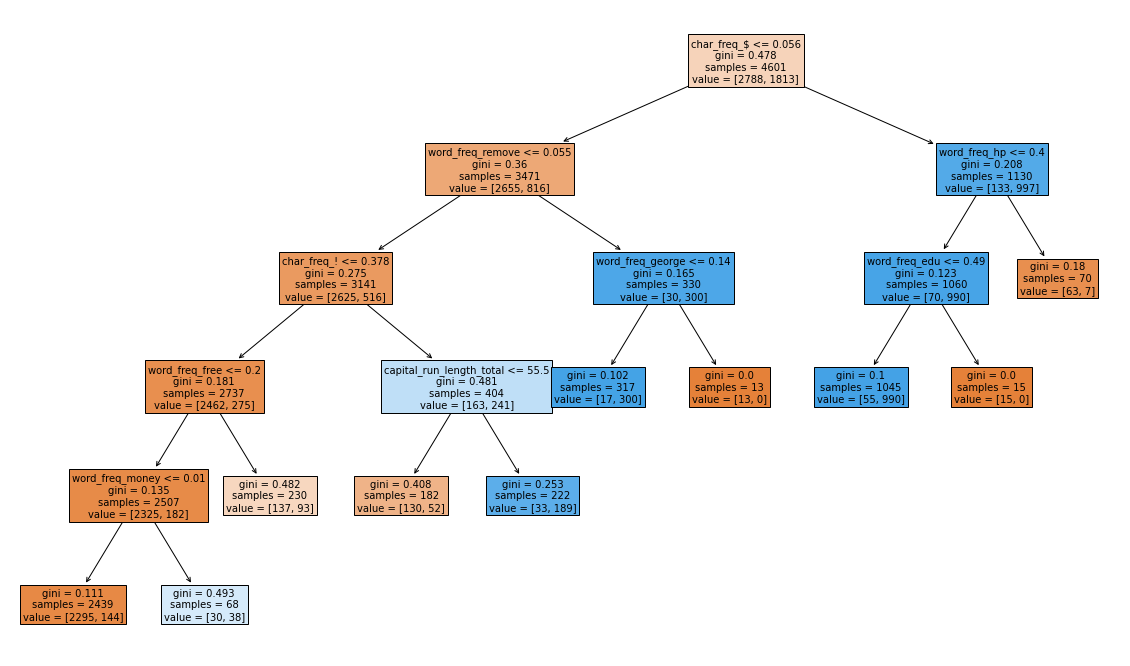
\includegraphics[width =1 \textwidth]{images/tree.png} 
\end{center}
\end{tcolorbox}

\item (15 points) Now also build a random forest model. Partition the data to use the first 80\% for training and the remaining 20\% for testing. Compare and report the test error for your classification tree and random forest models on testing data. Plot the curve of test error (total misclassification error rate) versus the number of trees for the random forest, and plot the test error for the CART model (which should be a constant with respect to the number of trees). 
\begin{tcolorbox}[breakable,enhanced]
\textbf{Solution:}
Firstly, I trained a random forest classifier with 100 random trees on the training set and obtained a test error of  6.08\%.  I also trained a decision tree classifier on the training set and obtained a test error of 9.45\%. \\

Then I trained 40 random forest classifiers, with number of random trees = 1, 6, 11, ..., 196, using the training set. Their test errors were shown in the following plot. As we can see, when the number of trees is around 75, the classifier achieved a very good performance. But when we increase the number of trees, the performance can not be greatly improved anymore. Given the small size of our dataset, if the number of random trees are very large, some of them may tend to be highly correlated with each other and provides no extra information. We can try AdaBoost to see if we can achieve a better performance. 
\begin{center}
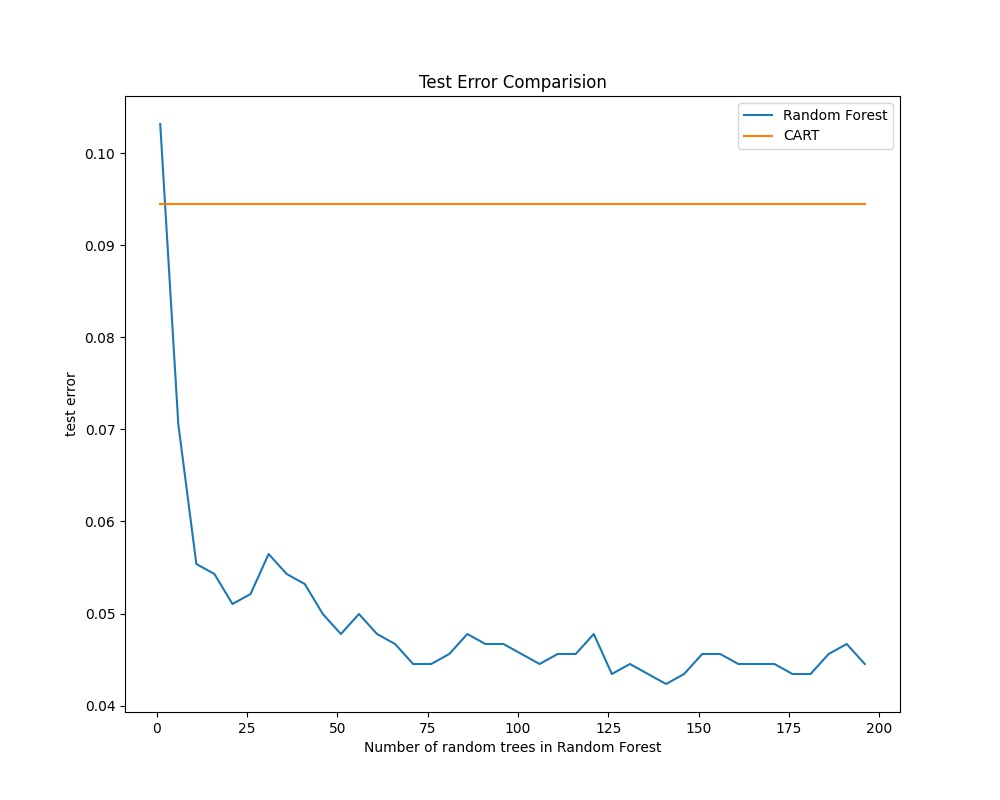
\includegraphics[width =.6 \textwidth]{images/test_error.jpg} 
\end{center}
\end{tcolorbox}

\item (15 points) Now we will use a one-class SVM approach for spam filtering. Partition the data to use the first 80\% for training and the remaining 20\% for testing. Extract all {\it non-spam} emails from the training block (80\% of data you have selected) to build the one-class kernel SVM using RBF kernel (you can turn the kernel bandwidth to achieve good performance). Then apply it on the 20\% of data reserved for testing (thus this is a novelty detection situation), and report the total misclassification error rate on these testing data. 
\begin{tcolorbox}[breakable,enhanced]
\textbf{Solution:}
The one-class SVM only uses the information of the non-spam emails in the training set. Unsurprisingly, it has a higher test compared with decision tree and random forest models. I fine tuned the parameter gamma for one-class SVM and found that 0.03 is the optimal gamma with the lowest test error 35.61\%. (The mean trick (test error 42.45\%) didn't work good here. )
\end{tcolorbox}

\end{enumerate}


\end{enumerate}





\end{document}
